\section{Customer}

\subsection{Signing out}
In order to sign out of \textit{EmporioLambda}, you must first be logged in. You will then see, in any page of the website, a 'Sign out' button. Press this button to be logged off the website.

\begin{figure}[H]
\makebox[\textwidth][c]{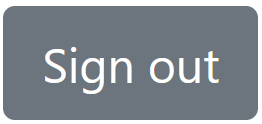
\includegraphics[width=1.2\textwidth]{res/Immagini/SignoutButton}}%
\caption{Page header with the sign out button}
\end{figure}

\subsection{Checkout}
To buy the products listed on \textit{EmporioLambda} you must first add them to your cart and be signed in as a customer. The checkout procedure starts in the cart page, where you'll have to click the 'Pay' button which is located under the total price of the items in the cart. This will lead you to a page where you'll have to insert the payment details for your order.

\begin{figure}[H]
\makebox[\textwidth][c]{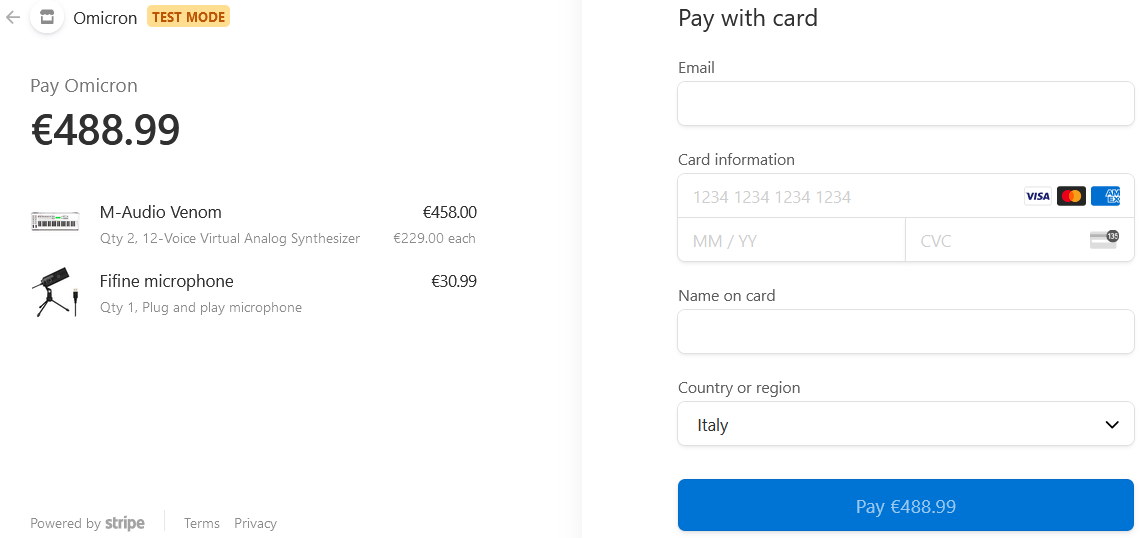
\includegraphics[width=1.2\textwidth]{res/Immagini/StripeCheckout}}%
\caption{Example of a checkout page}
\end{figure}

After inserting your credit card details and your email, click on the 'Pay' button to complete the order. If no errors happen during the payment process, you will receive an email containing your products and will be redirected to your user profile. The new order should now appear in your profile's order section. 

If any error occurs during the checkout procedure, you will be redirected to the previous section with an error message describing what the problem is. If the message isn't self explanatory, please refer to section 6 issue reporting.

\subsection{Viewing and modifying your user data}
To access your user data, navigate to the profile page by clicking on the 'Profile' link in the website header section. You will see a 'Profile section' listing all of your user information.

\begin{figure}[H]
\centering
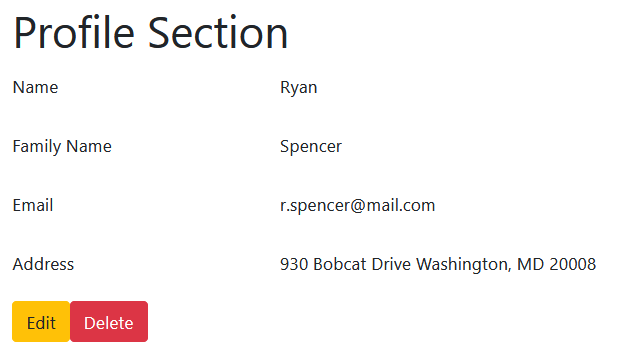
\includegraphics[scale=0.6]{res/Immagini/ProfilePage}
\caption{Example of a profile section}
\end{figure}

To edit any of your profile data, click on the 'Edit Profile' button. You will be redirected to a page with a form. Enter your updated information and click on the 'Submit' button to overwrite the previous data.

\begin{figure}[H]
\centering
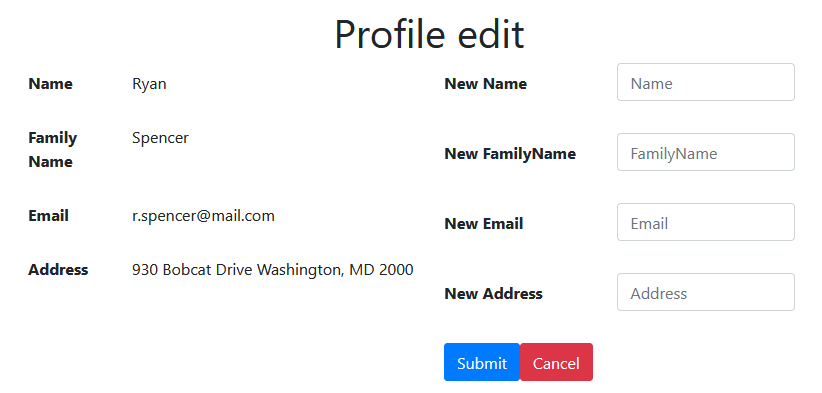
\includegraphics[scale=0.6]{res/Immagini/ProfileEdit}
\caption{Example of a profile edit page}
\end{figure}

\subsection{Modifying your password}
To edit your password, click on the 'Edit Password' button. A form will appear. Type your new password and click 'Submit' to update your profile password.

\begin{figure}[H]
\centering
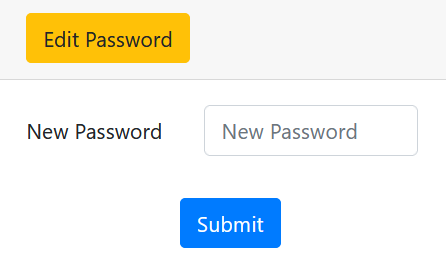
\includegraphics[scale=0.6]{res/Immagini/EditPassword}
\caption{Example of the password edit form}
\end{figure}

\subsection{Deleting your \textit{EmporioLambda} account}
To delete your account, access the profile page and click on the 'Delete' button. Your account will be deleted and you will be logged out.

\subsection{Viewing your previous orders}
To access a list of your previous orders, access the profile page. You will find, under the 'Profile section', an 'Orders section' containing all of your previous orders.

\begin{figure}[H]
\centering
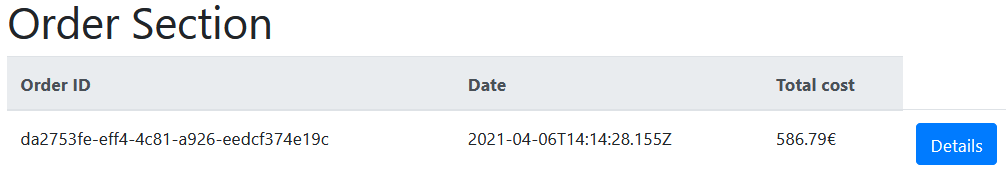
\includegraphics[scale=0.6]{res/Immagini/OrderSection}
\caption{Example of an orders list section}
\end{figure}

To see more information, click on the 'Details' button. You will be redirected to a page listing all of the order details.

\begin{figure}[H]
\centering
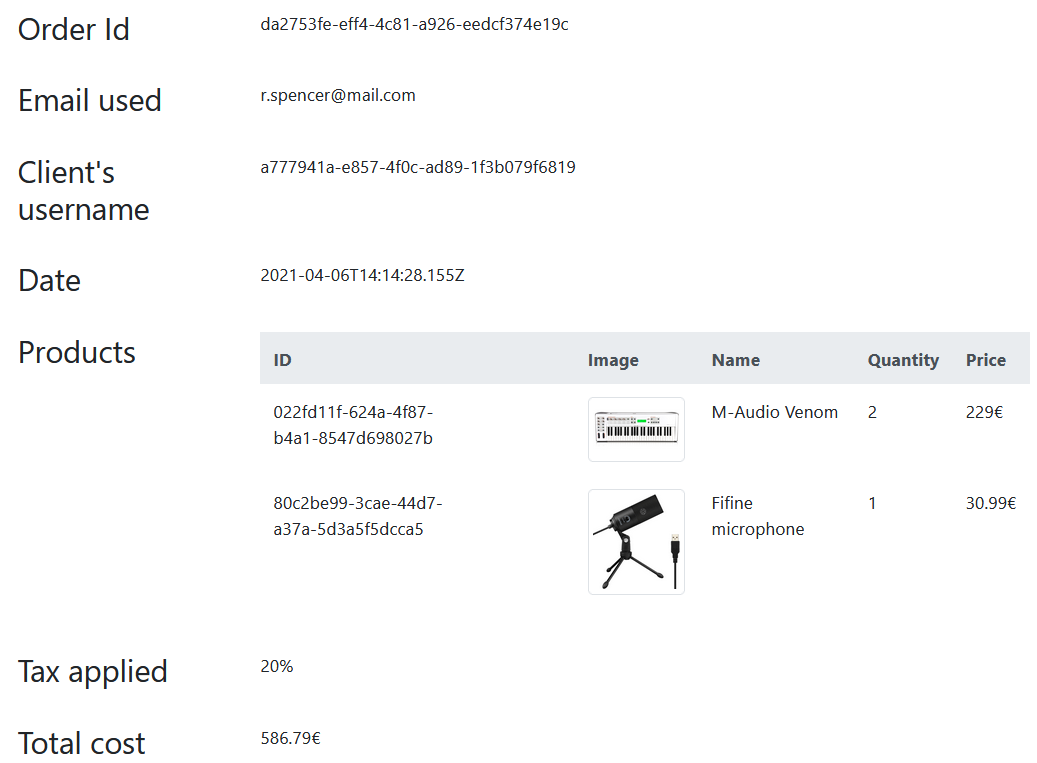
\includegraphics[scale=0.6]{res/Immagini/OrderDetails}
\caption{Example of an orders details page}
\end{figure}

